
\documentclass{article}
\usepackage{amsmath, amssymb, graphicx, geometry, tikz, array, booktabs, enumitem, listings, xcolor, fancyhdr, float, subcaption, hyperref}

\title{Module 6: Linear Boundaries for Binary Classification}
\author{Machine Learning Course}
\date{}

\begin{document}

\maketitle
\tableofcontents
\newpage

\section{Introduction to Linear Classification}

\subsection{From Regression to Classification}
In previous modules, we explored regression and conditional probability estimation, approaching each as an optimization task. We now extend this optimization mindset to classification problems, specifically focusing on linear boundaries for binary classification.

\subsection{The Classification Framework}
In binary classification:
\begin{itemize}
    \item Input: Feature vectors $x \in \mathbb{R}^d$
    \item Output: Binary labels $y \in \{-1, +1\}$
    \item Goal: Learn a decision boundary that separates positive from negative examples
\end{itemize}

\subsection{Linear vs. Non-linear Classification}
Linear classification uses a hyperplane to separate the feature space:
\begin{itemize}
    \item Simple, interpretable models
    \item Efficient to train and evaluate
    \item Limited expressivity (can only represent linearly separable patterns)
    \item Foundation for more complex models (e.g., neural networks)
\end{itemize}

\section{Geometry of Linear Classification}

\subsection{Linear Decision Boundaries in Two Dimensions}
A linear decision boundary in 2D is a line that separates the feature space into two regions.

\paragraph{Example: Line with y-intercept = 4, slope = -4/3}
\begin{align}
    x_2 &= -\frac{4}{3}x_1 + 4 \quad \text{(slope-intercept form)}\\
    \Rightarrow 4x_1 + 3x_2 - 12 &= 0 \quad \text{(standard form)}
\end{align}

\begin{figure}[h]
\centering
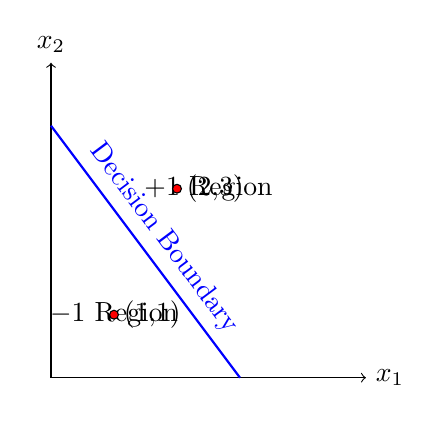
\begin{tikzpicture}[scale=0.8]
    \draw[->] (0,0) -- (5,0) node[right] {$x_1$};
    \draw[->] (0,0) -- (0,5) node[above] {$x_2$};
    \draw[thick, blue] (0,4) -- (3,0) node[midway, above, sloped] {Decision Boundary};
    \node at (2.5,3) {$+1$ Region};
    \node at (1,1) {$-1$ Region};
    \draw[fill=red] (2,3) circle (2pt) node[right] {(2,3)};
    \draw[fill=red] (1,1) circle (2pt) node[right] {(1,1)};
\end{tikzpicture}
\caption{A linear decision boundary in 2D space with positive and negative regions}
\end{figure}

\subsection{Making Predictions with Linear Boundaries}
To classify a point, we evaluate the linear function at that point:
\begin{itemize}
    \item If the result is positive, predict $+1$
    \item If the result is negative, predict $-1$
\end{itemize}

\paragraph{Example 1: Classifying the point (2,3)}
\begin{align}
    4x_1 + 3x_2 - 12 &= 4(2) + 3(3) - 12\\
    &= 8 + 9 - 12\\
    &= 5 > 0
\end{align}
Since the result is positive, we predict $+1$.

\paragraph{Example 2: Classifying the point (1,1)}
\begin{align}
    4x_1 + 3x_2 - 12 &= 4(1) + 3(1) - 12\\
    &= 4 + 3 - 12\\
    &= -5 < 0
\end{align}
Since the result is negative, we predict $-1$.

\section{Linear Classification in D-Dimensional Space}

\subsection{Mathematical Formulation}
In the general case with $d$-dimensional data:
\begin{itemize}
    \item Data points: $\mathbf{x} \in \mathbb{R}^d$
    \item Labels: $y \in \{-1, +1\}$
    \item Weight vector: $\mathbf{w} \in \mathbb{R}^d$
    \item Bias term: $b \in \mathbb{R}$
\end{itemize}

The decision boundary is defined by:
\[
\mathbf{w} \cdot \mathbf{x} + b = 0
\]

\subsection{Prediction Rule}
For a new point $\mathbf{x}$, the prediction is:
\[
\hat{y} = \text{sign}(\mathbf{w} \cdot \mathbf{x} + b) = 
\begin{cases}
+1 & \text{if } \mathbf{w} \cdot \mathbf{x} + b > 0\\
-1 & \text{if } \mathbf{w} \cdot \mathbf{x} + b < 0
\end{cases}
\]

\subsection{Correctness Condition}
A prediction is correct if and only if:
\begin{itemize}
    \item True label $y = +1$ and $\mathbf{w} \cdot \mathbf{x} + b > 0$, OR
    \item True label $y = -1$ and $\mathbf{w} \cdot \mathbf{x} + b < 0$
\end{itemize}

This can be expressed compactly as:
\[
y(\mathbf{w} \cdot \mathbf{x} + b) > 0
\]

\section{Geometric Interpretation}

\subsection{Properties of the Weight Vector}
The weight vector $\mathbf{w}$ has several important geometric properties:
\begin{itemize}
    \item $\mathbf{w}$ is perpendicular (normal) to the decision boundary
    \item The magnitude of $\mathbf{w}$ affects the "steepness" of the classifier but not the boundary itself
    \item The direction of $\mathbf{w}$ points toward the positive region
\end{itemize}

\begin{figure}[h]
\centering
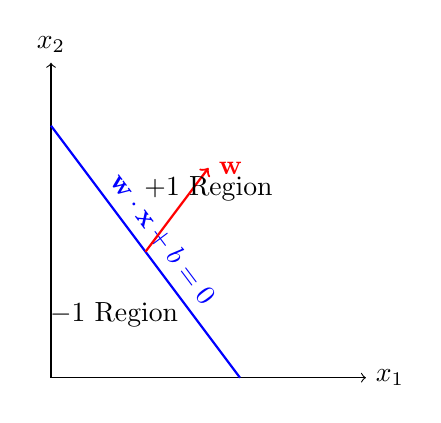
\begin{tikzpicture}[scale=0.8]
    \draw[->] (0,0) -- (5,0) node[right] {$x_1$};
    \draw[->] (0,0) -- (0,5) node[above] {$x_2$};
    \draw[thick, blue] (0,4) -- (3,0) node[midway, above, sloped] {$\mathbf{w} \cdot \mathbf{x} + b = 0$};
    \draw[->, thick, red] (1.5,2) -- (2.5,3.33) node[right] {$\mathbf{w}$};
    \node at (2.5,3) {$+1$ Region};
    \node at (1,1) {$-1$ Region};
\end{tikzpicture}
\caption{The weight vector $\mathbf{w}$ is perpendicular to the decision boundary}
\end{figure}

\subsection{Role of the Bias Term}
The bias term $b$ determines the offset of the decision boundary from the origin:
\begin{itemize}
    \item If $b = 0$, the boundary passes through the origin
    \item If $b > 0$, the boundary is shifted in the direction opposite to $\mathbf{w}$
    \item If $b < 0$, the boundary is shifted in the direction of $\mathbf{w}$
\end{itemize}

\subsection{Distance to the Decision Boundary}
The distance from a point $\mathbf{x}$ to the decision boundary is:
\[
d(\mathbf{x}) = \frac{|\mathbf{w} \cdot \mathbf{x} + b|}{\|\mathbf{w}\|}
\]

This has an important interpretation: points further from the boundary are classified with higher confidence.

\section{Learning Linear Classifiers}

\subsection{Optimization Perspective}
Learning a linear classifier involves finding the parameters $\mathbf{w}$ and $b$ that minimize a loss function. Different algorithms use different loss functions:

\begin{itemize}
    \item Perceptron: Uses a direct misclassification measure
    \item Logistic Regression: Uses log loss
    \item Support Vector Machines: Uses hinge loss
\end{itemize}

\subsection{The Perceptron Algorithm}
The perceptron is one of the earliest and most influential algorithms for linear classification.

\paragraph{Algorithm:}
\begin{enumerate}
    \item Initialize $\mathbf{w} = \mathbf{0}$, $b = 0$
    \item Repeat until convergence:
    \begin{enumerate}
        \item For each training example $(\mathbf{x}^{(i)}, y^{(i)})$:
        \begin{enumerate}
            \item If $y^{(i)}(\mathbf{w} \cdot \mathbf{x}^{(i)} + b) \leq 0$ (misclassified):
            \begin{enumerate}
                \item $\mathbf{w} \leftarrow \mathbf{w} + y^{(i)}\mathbf{x}^{(i)}$
                \item $b \leftarrow b + y^{(i)}$
            \end{enumerate}
        \end{enumerate}
    \end{enumerate}
\end{enumerate}

\paragraph{Convergence Property:}
If the data is linearly separable, the perceptron algorithm is guaranteed to converge to a solution in a finite number of steps.

\subsection{Logistic Regression for Linear Classification}
Logistic regression fits a linear boundary by modeling the probability of class membership:
\[
P(Y = +1 | \mathbf{x}, \mathbf{w}, b) = \frac{1}{1 + e^{-(\mathbf{w} \cdot \mathbf{x} + b)}}
\]

The decision boundary is still $\mathbf{w} \cdot \mathbf{x} + b = 0$, but the model provides probabilities rather than just binary predictions.

\subsection{Support Vector Machines (SVMs)}
SVMs find the linear boundary that maximizes the margin (distance to the closest points from each class):
\begin{align}
\min_{\mathbf{w}, b} \frac{1}{2}\|\mathbf{w}\|^2 \quad \text{subject to} \quad y^{(i)}(\mathbf{w} \cdot \mathbf{x}^{(i)} + b) \geq 1 \quad \forall i
\end{align}

\begin{figure}[h]
\centering
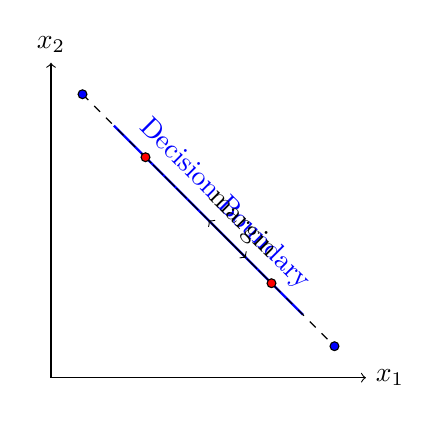
\begin{tikzpicture}[scale=0.8]
    \draw[->] (0,0) -- (5,0) node[right] {$x_1$};
    \draw[->] (0,0) -- (0,5) node[above] {$x_2$};
    \draw[thick, blue] (1,4) -- (4,1) node[midway, above, sloped] {Decision Boundary};
    \draw[dashed] (0.5,4.5) -- (3.5,1.5);
    \draw[dashed] (1.5,3.5) -- (4.5,0.5);
    \draw[<->] (2.5,2.5) -- (3.1,1.9) node[midway, above, sloped] {margin};
    \draw[fill=red] (1.5,3.5) circle (2pt);
    \draw[fill=red] (3.5,1.5) circle (2pt);
    \draw[fill=blue] (0.5,4.5) circle (2pt);
    \draw[fill=blue] (4.5,0.5) circle (2pt);
\end{tikzpicture}
\caption{SVM finds the decision boundary that maximizes the margin}
\end{figure}

\section{Limitations and Extensions}

\subsection{Linearly Non-separable Data}
When data is not linearly separable, several approaches can be used:
\begin{itemize}
    \item Soft-margin SVM: Allow some misclassifications with penalties
    \item Kernel methods: Implicitly map data to a higher-dimensional space where it becomes linearly separable
    \item Feature engineering: Create new features that make the data linearly separable
\end{itemize}

\subsection{The Kernel Trick}
The kernel trick allows us to implicitly work in a higher-dimensional space without explicitly computing the mapping:
\begin{itemize}
    \item Linear kernel: $K(\mathbf{x}, \mathbf{z}) = \mathbf{x} \cdot \mathbf{z}$
    \item Polynomial kernel: $K(\mathbf{x}, \mathbf{z}) = (\mathbf{x} \cdot \mathbf{z} + c)^d$
    \item RBF kernel: $K(\mathbf{x}, \mathbf{z}) = \exp(-\gamma\|\mathbf{x} - \mathbf{z}\|^2)$
\end{itemize}

\subsection{Multi-class Classification}
Binary classification can be extended to multi-class problems using:
\begin{itemize}
    \item One-vs-Rest: Train $k$ binary classifiers, each separating one class from the rest
    \item One-vs-One: Train $\binom{k}{2}$ binary classifiers, one for each pair of classes
    \item Direct multi-class formulations (e.g., multinomial logistic regression)
\end{itemize}

\section{Worked Examples}

\subsection{Example 1: Finding the Decision Boundary}
Given points $(1,2)$ labeled $+1$ and $(2,1)$ labeled $-1$, find a linear decision boundary.

\paragraph{Solution:}
We need to find $w_1$, $w_2$, and $b$ such that:
\begin{align}
w_1 \cdot 1 + w_2 \cdot 2 + b &> 0 \quad \text{(for the $+1$ point)}\\
w_1 \cdot 2 + w_2 \cdot 1 + b &< 0 \quad \text{(for the $-1$ point)}
\end{align}

One possible solution is $w_1 = -1$, $w_2 = 1$, $b = 0$:
\begin{align}
-1 \cdot 1 + 1 \cdot 2 + 0 &= 1 > 0 \quad \checkmark\\
-1 \cdot 2 + 1 \cdot 1 + 0 &= -1 < 0 \quad \checkmark
\end{align}

The decision boundary is $-x_1 + x_2 = 0$ or $x_2 = x_1$.

\subsection{Example 2: Perceptron Algorithm Trace}
Consider the dataset:
\begin{itemize}
    \item $(1,1)$ with label $+1$
    \item $(0,1)$ with label $+1$
    \item $(0,0)$ with label $-1$
    \item $(1,0)$ with label $-1$
\end{itemize}

\paragraph{Perceptron Trace:}
\begin{enumerate}
    \item Initialize $\mathbf{w} = (0,0)$, $b = 0$
    \item First example $(1,1)$, $y = +1$:
    \begin{align}
    y(\mathbf{w} \cdot \mathbf{x} + b) &= 1 \cdot ((0,0) \cdot (1,1) + 0) = 0 \leq 0
    \end{align}
    Misclassified, so update:
    \begin{align}
    \mathbf{w} &\leftarrow (0,0) + 1 \cdot (1,1) = (1,1)\\
    b &\leftarrow 0 + 1 = 1
    \end{align}
    
    \item Second example $(0,1)$, $y = +1$:
    \begin{align}
    y(\mathbf{w} \cdot \mathbf{x} + b) &= 1 \cdot ((1,1) \cdot (0,1) + 1) = 2 > 0
    \end{align}
    Correctly classified, no update.
    
    \item Third example $(0,0)$, $y = -1$:
    \begin{align}
    y(\mathbf{w} \cdot \mathbf{x} + b) &= -1 \cdot ((1,1) \cdot (0,0) + 1) = -1 < 0
    \end{align}
    Correctly classified, no update.
    
    \item Fourth example $(1,0)$, $y = -1$:
    \begin{align}
    y(\mathbf{w} \cdot \mathbf{x} + b) &= -1 \cdot ((1,1) \cdot (1,0) + 1) = -2 < 0
    \end{align}
    Correctly classified, no update.
\end{enumerate}

After one pass through the data, all examples are correctly classified. The final decision boundary is $x_1 + x_2 + 1 = 0$ or $x_2 = -x_1 - 1$.

\section{Connection to Neural Networks}

\subsection{The Perceptron as a Building Block}
The perceptron can be viewed as a single neuron in a neural network:
\begin{itemize}
    \item Inputs: $\mathbf{x} = (x_1, x_2, \ldots, x_d)$
    \item Weights: $\mathbf{w} = (w_1, w_2, \ldots, w_d)$
    \item Bias: $b$
    \item Activation function: $\text{sign}(z)$
    \item Output: $\hat{y} = \text{sign}(\mathbf{w} \cdot \mathbf{x} + b)$
\end{itemize}

\subsection{From Linear to Non-linear Classification}
Neural networks extend the perceptron by:
\begin{itemize}
    \item Using multiple layers of neurons
    \item Employing non-linear activation functions (e.g., sigmoid, ReLU)
    \item Learning hierarchical representations of the data
\end{itemize}

\begin{figure}[h]
\centering
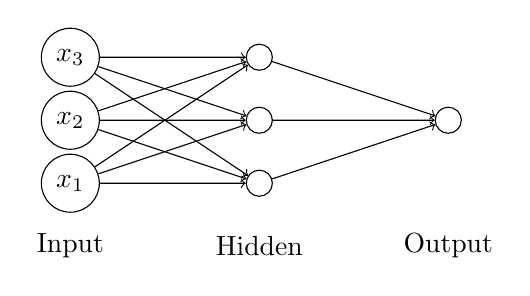
\begin{tikzpicture}[scale=0.8]
    % Input layer
    \foreach \i in {1,2,3} {
        \node[circle, draw] (I\i) at (0,\i) {$x_\i$};
    }
    \node at (0,0) {Input};
    
    % Hidden layer
    \foreach \i in {1,2,3} {
        \node[circle, draw] (H\i) at (3,\i) {};
    }
    \node at (3,0) {Hidden};
    
    % Output layer
    \node[circle, draw] (O1) at (6,2) {};
    \node at (6,0) {Output};
    
    % Connections
    \foreach \i in {1,2,3} {
        \foreach \j in {1,2,3} {
            \draw[->] (I\i) -- (H\j);
        }
    }
    
    \foreach \i in {1,2,3} {
        \draw[->] (H\i) -- (O1);
    }
\end{tikzpicture}
\caption{A simple neural network with one hidden layer}
\end{figure}

\section{Practical Considerations}

\subsection{Feature Scaling}
Linear classifiers are sensitive to the scale of features. Common scaling techniques include:
\begin{itemize}
    \item Min-max scaling: $x' = \frac{x - \min(x)}{\max(x) - \min(x)}$
    \item Standardization: $x' = \frac{x - \mu}{\sigma}$
\end{itemize}

\subsection{Regularization}
To prevent overfitting, regularization terms can be added to the optimization objective:
\begin{itemize}
    \item L1 regularization: $\lambda \|\mathbf{w}\|_1$ (promotes sparsity)
    \item L2 regularization: $\lambda \|\mathbf{w}\|_2^2$ (prevents large weights)
\end{itemize}

\subsection{Evaluation Metrics}
Common metrics for binary classification include:
\begin{itemize}
    \item Accuracy: $\frac{\text{Correct predictions}}{\text{Total predictions}}$
    \item Precision: $\frac{\text{True positives}}{\text{True positives + False positives}}$
    \item Recall: $\frac{\text{True positives}}{\text{True positives + False negatives}}$
    \item F1 Score: $2 \cdot \frac{\text{Precision} \cdot \text{Recall}}{\text{Precision} + \text{Recall}}$
    \item Area Under ROC Curve (AUC)
\end{itemize}

\section{Summary and Key Takeaways}

\subsection{Core Concepts}
\begin{itemize}
    \item Linear classifiers separate the feature space using a hyperplane
    \item The decision boundary is defined by $\mathbf{w} \cdot \mathbf{x} + b = 0$
    \item Predictions are made based on the sign of $\mathbf{w} \cdot \mathbf{x} + b$
    \item A prediction is correct when $y(\mathbf{w} \cdot \mathbf{x} + b) > 0$
\end{itemize}

\subsection{Algorithms}
\begin{itemize}
    \item Perceptron: Simple, iterative algorithm for linearly separable data
    \item Logistic Regression: Probabilistic approach to linear classification
    \item Support Vector Machines: Maximum-margin linear classifiers
\end{itemize}

\subsection{Extensions}
\begin{itemize}
    \item Kernel methods for non-linear classification
    \item Multi-class classification techniques
    \item Neural networks as generalizations of perceptrons
\end{itemize}

\subsection{Practical Tips}
\begin{itemize}
    \item Scale features appropriately
    \item Use regularization to prevent overfitting
    \item Choose evaluation metrics based on the problem context
    \item Consider non-linear methods if data is not linearly separable
\end{itemize}

\end{document}
